\documentclass{deliverablereport}
\usepackage{wrapfig}

\deliverable{UI}{ipython-advanced-interacts}
\deliverydate{31/08/2018}
\duedate{31/08/2018 (M36)}
\author{Odile Bénassy and Nicolas M. Thiéry}

\begin{document}
\maketitle
% This will be the abstract, fetched from the github description
\githubissuedescription

\section{Introduction}

\TODO{Write a one (half) page summary of this introduction, and put it
  in the github description}

The \href{https://jupyter.org}{Jupyter Notebook} is a web application
that enables the creation and sharing of executable documents
containing live code, equations, visualizations and explanatory text.
Reaching far beyond the standard
\href{https://en.wikipedia.org/wiki/Read-eval-print_loop}{REPL}
interaction (Read-Eval-Print Loop), a key feature of Jupyter is its
\href{http://jupyter.org/widgets}{Interactive widgets} which enable
real time interactive data visualizations; the Jupyter community has
developed a large array of widgets for interactive 2D and 3D
visualization of data in the form of charts, maps, tables, etc; see
e.g. \delivref{UI}{vis3d} for ODK's contribution to 3D visualization.
Furthermore, widgets can be \emph{composed} to build rich
applications, with all the usual UI components (e.g. menus, sliders,
or layout control).

\begin{figure}[h]\begin{center}
  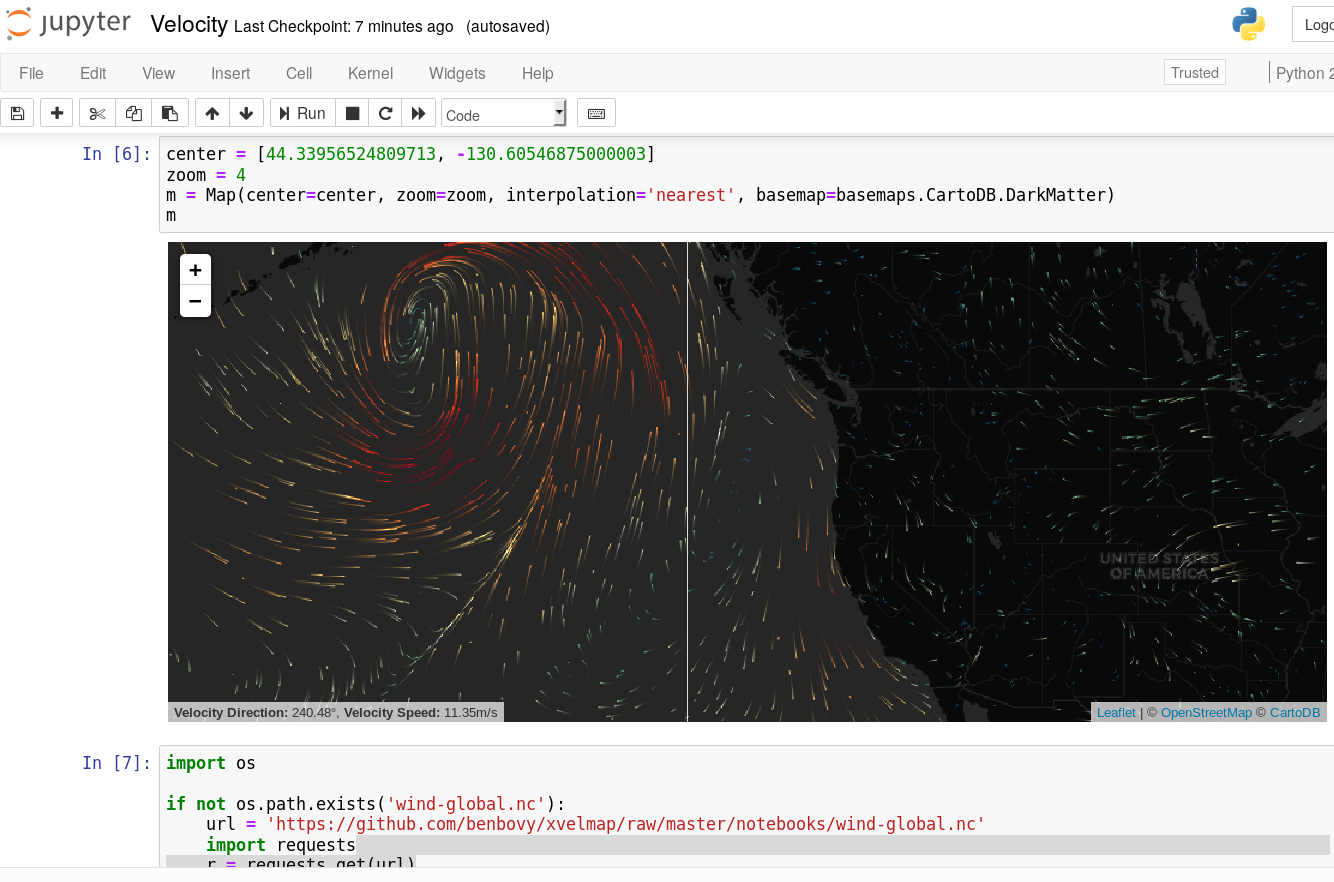
\includegraphics[width=\textwidth]{images/Velocity}
\end{center}\end{figure}

\TODO{screenshots: e.g. ipyleaflet + some application (exple appli web)}

\newpage

Hence, the Jupyter stack provides a very flexible environment catering
for use cases ranging from a novice users typing just a few commands
or browsing interactive documents to more advanced users authoring
rich interactive applications for their fellows.

The question we are tackling in this report is how this technology --
and specifically Jupyter widgets -- can be leveraged for pure
mathematics. The unique challenge comes from the huge variety of
mathematical objects that the user may want to visualize and
manipulate, some even coming with several natural ways to be
represented.

%\newpage

\begin{figure}[h]\begin{center}
    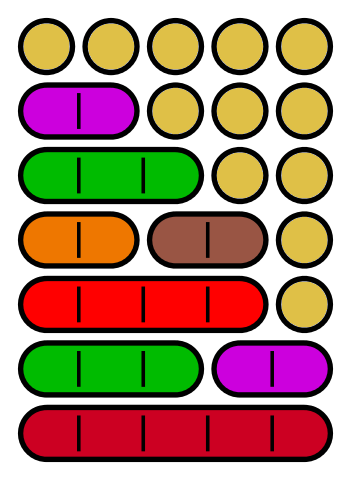
\includegraphics[width=0.20\textwidth]{images/partitions-of-5}
    \hspace{24px}
  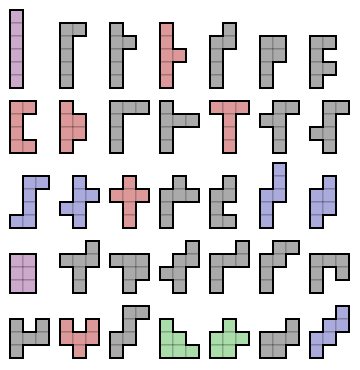
\includegraphics[width=0.25\textwidth]{images/hexominoes}
    \hspace{4px}
  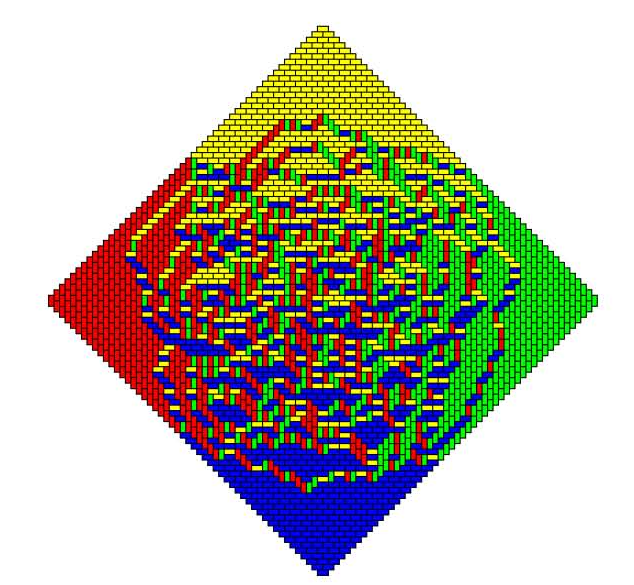
\includegraphics[width=0.36\textwidth]{images/AztecDiamond}
\end{center}\end{figure}\begin{figure}[h]\begin{center}
    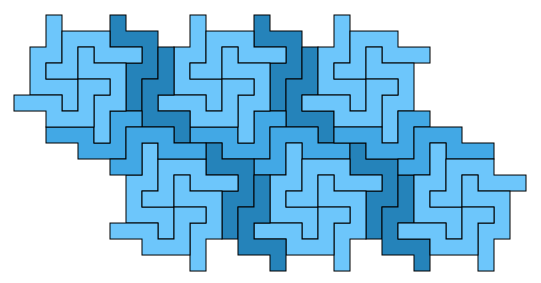
\includegraphics[width=0.4\textwidth]{images/nonominoes}
    \hspace{32px}
  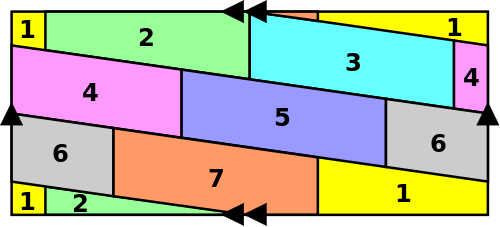
\includegraphics[width=0.4\textwidth]{images/500px-Torus_with_seven_colours}
\end{center}\end{figure}\begin{figure}[h]\begin{center}
  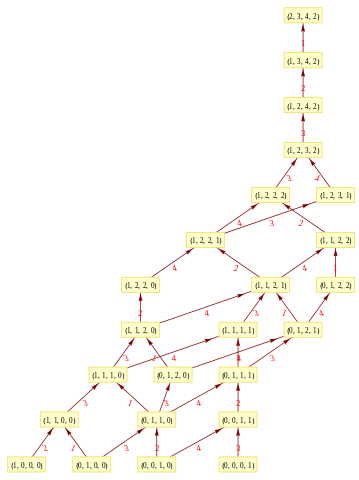
\includegraphics[width=0.3\textwidth]{images/359px-F4HassePoset}
    \hspace{4px}
  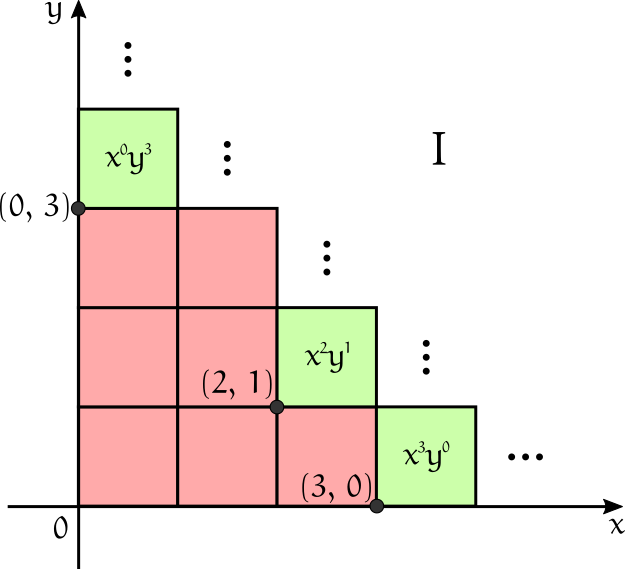
\includegraphics[width=0.3\textwidth]{images/Wikipic}
    \hspace{4px}
  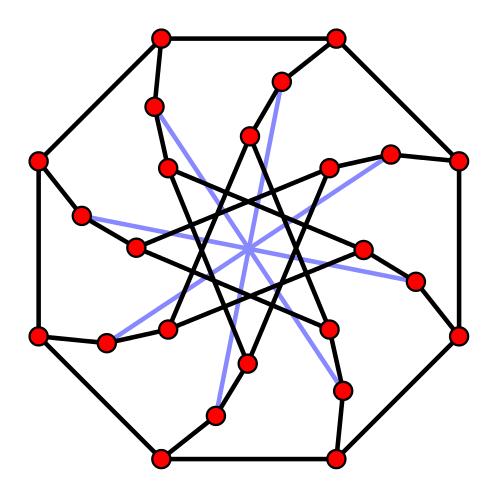
\includegraphics[width=0.3\textwidth]{images/500px-McGee_graph}
\end{center}\end{figure}\begin{figure}[h]\begin{center}
  
\includegraphics[width=0.3\textwidth]{images/fractioncont}
    \hspace{4px}
  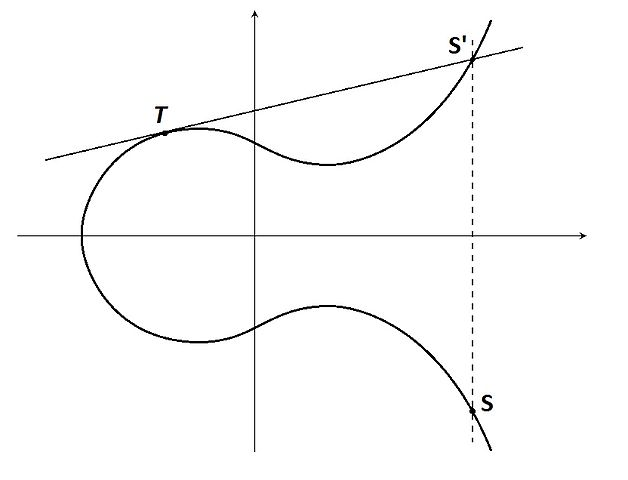
\includegraphics[width=0.3\textwidth]{images/elliptic-curve}
    \hspace{4px}
  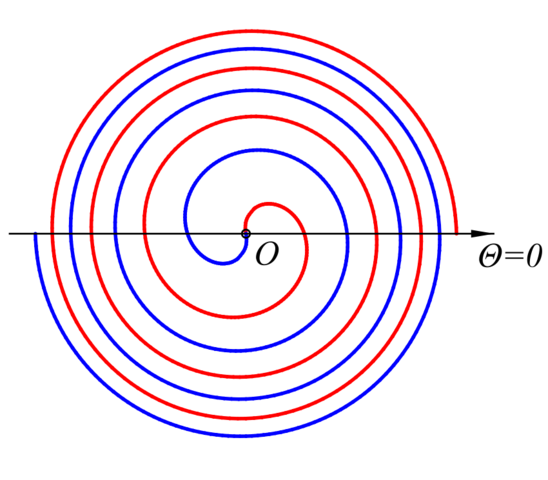
\includegraphics[width=0.3\textwidth]{images/548px-Fermat's_spiral_01}
\end{center}\end{figure}\begin{figure}[h]\begin{center}
  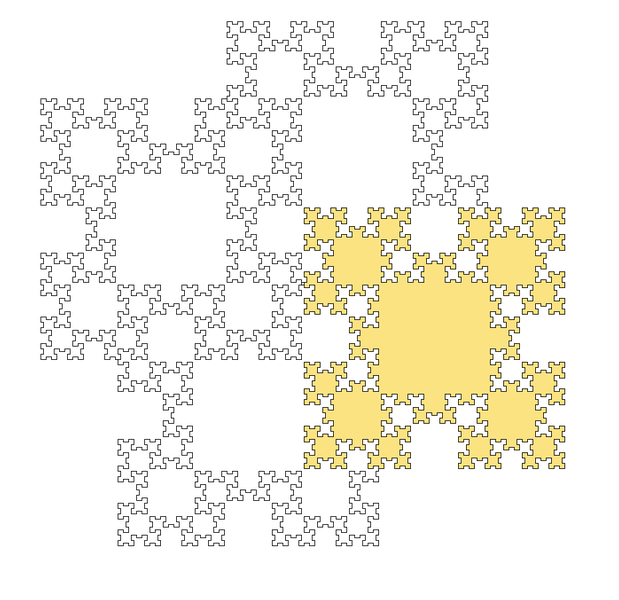
\includegraphics[width=0.3\textwidth]{images/619px-Tiling_Fibonacci_word_fractal}
    \hspace{32px}
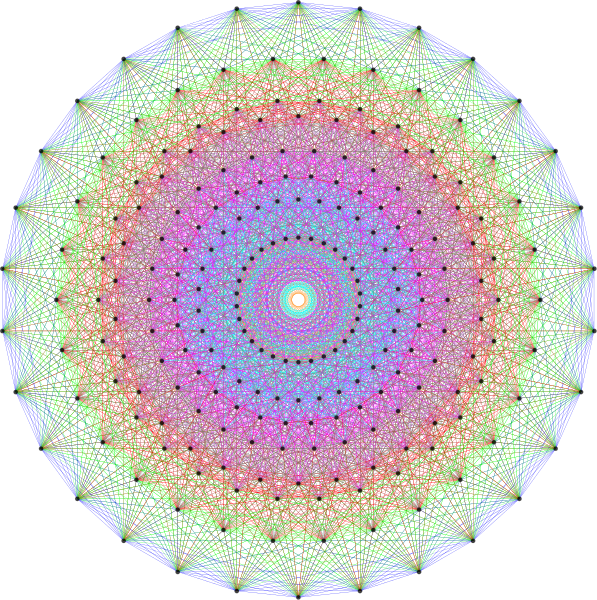
\includegraphics[width=0.3\textwidth]{images/597px-E8Petrie}
\end{center}\end{figure}

%\TODO{search on wikipedia for a nice collection of pictures: a
%  partition, a polyomino, an aztec diamond, a monomial ideal, a graph,
%  a poset, a formula - fraction continue, a curve, ...}. diagramme de Venn ; th des 4 couleurs sur une carte mathématique

\newpage

We therefore can't hope to provide hand crafted solutions for each
situation; instead we need to devise a toolbox of generic solutions
from which users can easily derive specialized visualizations for
their own pet objects.

We pursue two directions.

In the first one, we explore the development of widgets for the
graphical visualization of combinatorial objects.
The choice of this area of mathematics was, to some extent
out of personal interest and expertise, but more importantly because
devising good representations -- mental images -- of discrete objects
is at the heart of research in combinatorics. In Section~\ref{grid},
we report on the implementation in SageMath of a generic widget for
objects that admit a representation as a collection of cells on a 2D
grid, and specializations for typical objects such as partitions,
tableaux, polyominos, aztec diamonds, mazes.

\TODO{screenshot(s) of widgets displaying all of the above}

Another natural use case in combinatorics -- or more generally
discrete mathematics -- are objects that admit a graph-like
representation (trees, graphs, lattices of subgroups, crystals,
posets, discrete markov chains, to name a few). This use case is being
explored by the authors of the GAP package
\href{https://github.com/mcmartins/francy}{francy} under the
supervision(?) of ODK's member Markus Pfeiffer. Although ODK's
contribution in this direction is lightweight(?) at this stage, we
briefly report in Section~\ref{francy} on this use case to highlight
the lessons learned there and describe upcoming collaboration toward
bringing francy\'s features to SageMath.

In a second direction, we explore the use of Jupyter widgets not only
for the graphical visualization of an object, but for displaying a
page offering a synthetic overview of the information about that
object, including type, important properties and invariants, available
operations, related objects, documentation, etc. All sort of
information that is readily available by introspection but that a UI
can make easy to discover and emphasize according to relevance. The
challenge is that, given the huge variety of objects in a system like
SageMath, we can't afford to hand craft such pages for each type of
objects. In Section~\ref{sage-explorer} we report on our prototype
\lstinline{sage-explorer} that exploits the semantic embedded into the
system to produce a reasonable overview page automatically tailored to
each object.

\TODO{Screenshot of Sage-explorer?}

\TODO{Conclusion}

Altogether, the Jupyter Widget technology has proven as mature and
flexible as we hoped for. Designing new widgets does take some
expertise, but from the experience we gained, we are confident that it
lends itself well to the implementation of generic widgets by power
users that can be specialized by casual users and used by novices.

There remains two main challenges:
\begin{itemize}
\item How to best design widgets so that they can be reused across
  systems written in different languages? \TODO{Explain the tension
    kernel language / javascript}. \TODO{This will be explored by ... }
\item Widgets, as all modern web technologies, rely a lot on
  asynchronous execution. This is quite a different model from the
  Read-Eval-Print main loop that many not-so-young computational
  systems (including SageMath!) have originally been designed for, and
  such systems don't always behave well under asynchronous pressure:
  we have faced some bad crashes. How deep is the difficulty? How hard
  will it be to resolve it?
\end{itemize}

\section{State of the art}

\TODO{A standalone section? Or comments about it in the intro and along the way?}

In addition to the interactive widgets already delivered with ipywidgets (e.g. Sliders), numerous investigations, towards these goals, have been conducted in mathematical environments.

\begin{itemize}
\item The \href{http://www.lmfdb.org/}{LFMDB} database displays a comprehensive view of L-functions and Modular Forms in a web browser, yet still missing manipulation possibilities on the objects.
\item In the \href{https://core.ac.uk/download/pdf/9839511.pdf}{The
  Larch Environment} document (2013), Geoffrey W. French presents a visual
  interactive programming environment in Python language.
  One of his main ideas is to
  \emph{coerce} objects into graphical representations. Meaning that
  every object must know how it can be graphically represented, this
  representation being the default one and can be tailored by the
  user: G.W. French speaks of different \emph{perspectives} for the
  same object. The Larch Environment also maintains a state of objects
  in order to automatically refresh the representation.
%lists numerous tools editing or programming environments that existed back in 2012 for various programming languages. These included object editing or programming environments, some structured source code editors, and of course Sage with IPython.
\item Already within \href{http://mupad-combinat.sourceforge.net}{MuPAD-Combinat} project, an API was developed for a graphical representation combinatorial objects and their properties ; see \href{http://mupad-combinat.sourceforge.net/doc/en/Cat_Combinat/CombinatorialClassWith2DBoxedRepresentation.html}{Combinatorial Class With 2DBoxedRepresentation}. Yet that was only text-graphics i.e. ``ASCII art''.
\end{itemize}


\section{A generic widget for objects with a grid-like representation}
\label{grid}

\TODO{better liant?}

\begin{wrapfigure}{r}{0.25\textwidth}
    \begin{center}
      
\includegraphics[width=100px]{images/gridwidget}
      %\caption{A grid widget}
\end{center}
\end{wrapfigure}

We decided to first implement a generic widget meant for all SAGE-objects that can
be grid-like represented, the simplest one being a grid graph:

This use case combined several advantages:
\begin{itemize}
\item The UI part was relatively straightforward, for example
  requiring no Javascript side extension;
\item Little mathematical background was required; this, together with
  the previous point, made for a smooth learning curve for our
  Research Software Engineer;
\item It was a low hanging fruit with a large coverage;
\item The end result is immediately useful to colleagues, enabling
  early feedback from users;
\item There is a large variety of potential specializations, each with
  it's own quirks and specifics.
\end{itemize}
Hence, this use case provided a unique challenge: all the difficulty
resided in the the design of a generic solution that encapsulates as
much of the technicalities as possible, enabling users to specialize
the generic solution for their own pet objects with little expertise.

\TODO{Description of the design, of the API that subclasses must
  implement, code examples}

\TODO code and commit something more appropriate, given recent discussions

\TODO{potential applications}

\begin{wrapfigure}{r}{0.25\textwidth}
    \begin{center}
      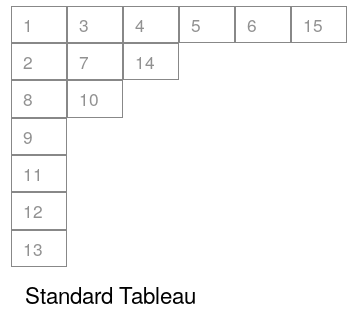
\includegraphics[width=100px]{images/tableauwidget}
      %\caption{A tableau widget}
\end{center}
\end{wrapfigure}

This generic widget can be used directly to represent grid graphs and
aztec diamond graphs. It is currently subclassed for partitions
and tableaus, with a support for \emph{editing cells and computing the
tableau subtype}, i.e. semi-standard or standard, where relevant. It
will soon support \emph{adding and deleting cells}, too.

The same GridWidget is also used to represent \emph{matchings} in grid-like
graphs.

\TODO{an image with dominos}

The code is distributed as a Sage package
\href{https://github.com/sagemath/sage-combinat-widgets/}{sage-combinat-widgets}
which is meant to grow beyond this initial seed, attracting
contributions from the community, and presumably be integrated
progressively into SageMath.

\TODO{Strategy to get feedback from users?}

\section{francy: an Interactive Discrete Mathematics Framework for GAP}

\TODO{Description of Francy: features, devs, ...}

\TODO{Francy is meant to become kernel-agnostic}

\TODO{How we plan to collaborate}

\section{Sage-explorer}
\label{sage-explorer}


\TODO{Screenshot of http://www.lmfdb.org/EllipticCurve/Q/11/a/2}
\TODO{Comparative screenshot of the same curve in sage-explorer}

\TODO{A bunch of screenshots}

\TODO{Description of the features}

\TODO{Description of how the page is built}

\TODO{Upcoming work}

\TODO{Strategy to get feedback from users?}

\appendix

\TODO{The demo notebooks?}



\end{document}

%%% Local Variables:
%%% mode: latex
%%% TeX-master: t
%%% End:

